\documentclass[a4paper]{article}
\usepackage{times}
\usepackage[utf8]{inputenc}
\usepackage[T1]{fontenc}
\usepackage{graphicx}
\usepackage{amssymb}
\usepackage{hyperref}
\linespread{1.5}	% double spaces lines
\usepackage[hmargin=3cm,vmargin=3cm]{geometry}
\usepackage{indentfirst}
\usepackage{amsmath}
\usepackage{amsthm}
\usepackage{sectsty}
\usepackage{enumitem}
\usepackage[brazil]{babel}
\usepackage{placeins} %mantem figuras na secao com \FloatBarrier
\usepackage{fixltx2e} %\textsubscript
\usepackage{textcomp}
\hypersetup{%
    pdfborder = {0 0 0}
}

\begin{document}

\begin{titlepage}
\begin{center}


\large{ 
\uppercase{ Universidade Federal do Rio Grande do Sul\\

Instituto de Informática \\

Curso de Ciência da Computação \\

Circuitos Digitais (2014/1)\\
}

Prof. Dr. Marcelo de Oliveira Johann \\

Graduandos: \\ Paulo Renato Lanzarin (228818)
			\\ Ricardo Gabriel Herdt (160622) \\ [4.5cm]


% Title
\LARGE {\bfseries Relatório do laboratório 06: \\
	Projeto de decodificador para 7 segmentos\\[1.0cm]
}}


\vfill

Porto Alegre, 24 de abril de 2014

\end{center}
\end{titlepage}
\section{Descrição}

	O projeto deste laboratório consistiu na elaboração de um decodificador
para 7 segmentos. Mais precisamente, os 4 bits de entrada são decodificados
para o correspondente dígito de 0 a 9 (os quais são "desenhados" em segmentos
de LED's enumerados de 'a' a 'g'). Para tanto, a partir de uma tabela verdade
construída relacionando cada valor de entrada com os segmentos acionados,
minimizou-se a correspondente função booleana através de mapas de Karnaugh e
construiu-se o circuito.



\FloatBarrier
\section{Tabela Verdade}

	As funções de decodificação para ativação de cada LED (obtidas a partir da minimização por mapa de Karnaugh através dos valores da tabela-verdade acima) e a montagem dos circuitos especificos são como seguem nas subseções.



\begin{table}[h]
\centering
\begin{tabular}{| *{9}{c |}}%{| *{9}{p{0.6cm} |} }
	\hline
	n\textordmasculine	&$i_3i_2i_1i_0$	&a &b &c &d &e &f &g \\
	0 &0000 &1 &1 &1 &1 &1 &1 &0 \\
	1 &0001 &0 &1 &1 &0 &0 &0 &0 \\
	2 &0010 &1 &1 &0 &1 &1 &0 &1 \\
	3 &0011 &1 &1 &1 &1 &0 &0 &1 \\
	4 &0100 &0 &1 &1 &0 &0 &1 &1 \\
	5 &0101 &1 &0 &1 &1 &0 &1 &1 \\
	6 &0110 &1 &0 &1 &1 &0 &1 &1 \\
	7 &0111 &1 &1 &1 &0 &0 &0 &0 \\
	8 &1000 &1 &1 &1 &1 &1 &1 &1 \\
	9 &1001 &1 &1 &1 &0 &0 &1 &1 \\ 
	\hline
\end{tabular}
\caption{Tabela verdade}
\end{table}

\section{Equações minimizadas}

$a: i_2.i_0 + i_1 + i_3 + \neg i_2.\neg i_0$

$b: \neg i_3.\neg i_2 + \neg i_1.\neg i_0 + i_3 + i_1.i_0$

$c: i_0 + \neg i_1 + i_2 + i_3$

$d: \neg i_2.\neg i_0 + i_2.\neg i_1.i_0 + \neg i_2.i_1 + i_1.i_0$

$e: \neg i_2.\neg i_0 + i_1.~i_0$

$f: \neg i_1.\neg i_0 + i_3 + \neg i_3.i_2.\neg i_0 + \neg i_3.i_2.\neg i_1$

$g: i_1.\neg i_0 + i_2.\neg i_1 + i_3 + \neg i_2.i_1$

\FloatBarrier

\section{Circuitos}

	O decodificador de 7 segmentos foi projetado em blocos no programa \emph{Max+plus II}. Foram dispostas entradas de i0 a i3 que são conectadas em decodificadores menores projetados especificamentes para as funções de cada LED e que levam cada um a uma saída (que consistem dos correspondentes LEDs do dígito).
	A tabela verdade do decodificador é como segue, com 0-9 representando os dígitos que são ativados e a-g representando os LEDs correspondentes do dígito.



\begin{figure}[h!]
  \centering
  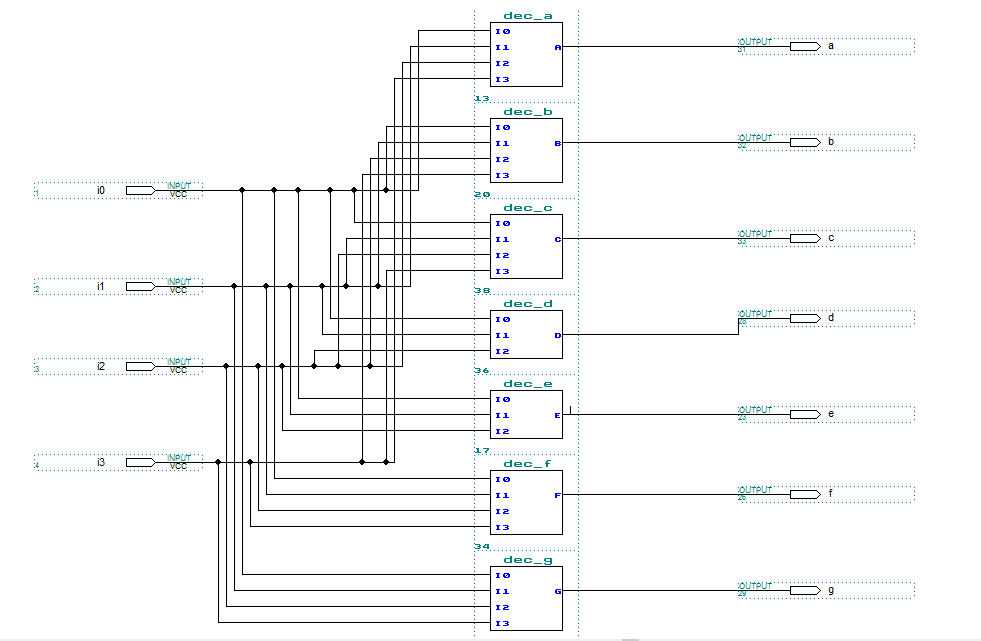
\includegraphics[scale=0.7]{dec_4-7.png}
  \caption{Visão geral do circuito}
\end{figure}


\begin{figure}[h!]
  \centering
  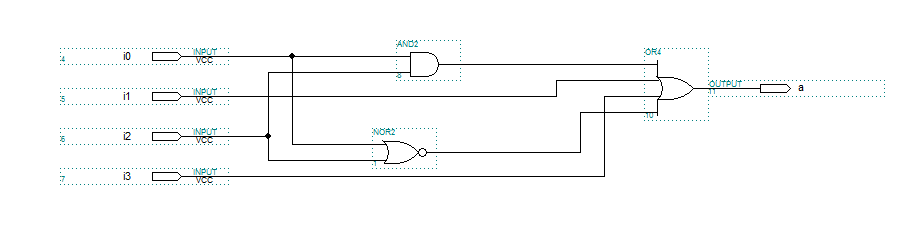
\includegraphics[scale=0.7]{dec_a.png}
  \caption{Decodificador 'a'}
\end{figure}

\begin{figure}[h!]
  \centering
  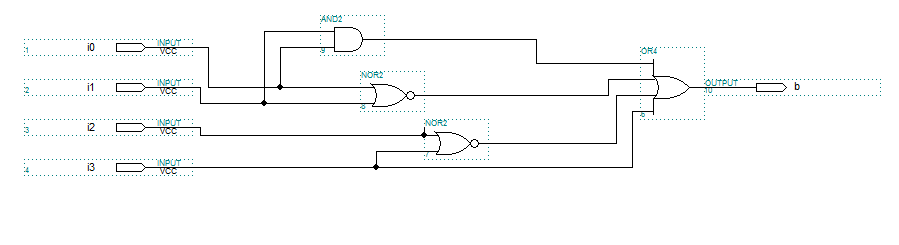
\includegraphics[scale=0.7]{dec_b.png}
  \caption{Decodificador 'b'}
\end{figure}

\begin{figure}[h!]
  \centering
  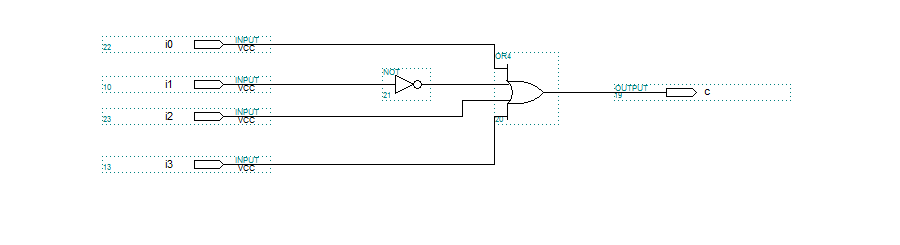
\includegraphics[scale=0.7]{dec_c.png}
  \caption{Decodificador 'c'}
\end{figure}

\begin{figure}[h!]
  \centering
  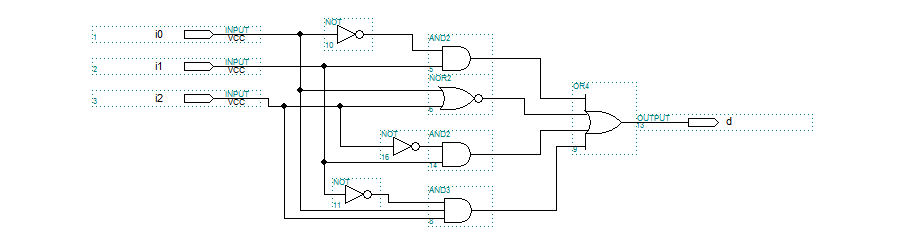
\includegraphics[scale=0.7]{dec_d.png}
  \caption{Decodificador 'd'}
\end{figure}

\begin{figure}[h!]
  \centering
  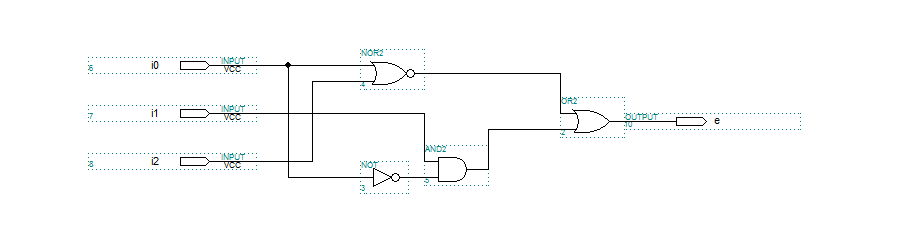
\includegraphics[scale=0.7]{dec_e.png}
  \caption{Decodificador 'e'}
\end{figure}

\begin{figure}[h!]
  \centering
  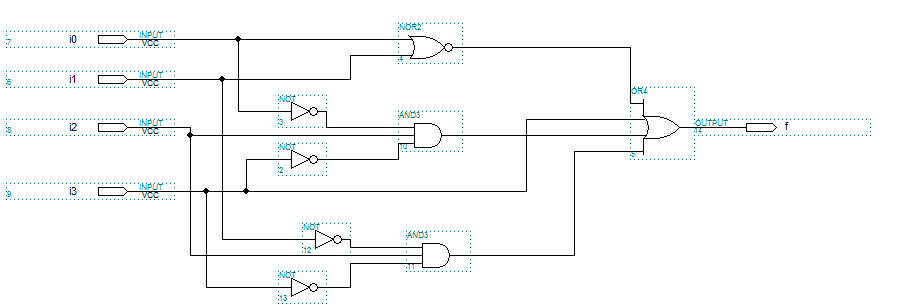
\includegraphics[scale=0.7]{dec_f.png}
  \caption{Decodificador 'f'}
\end{figure}

\begin{figure}[h!]
  \centering
  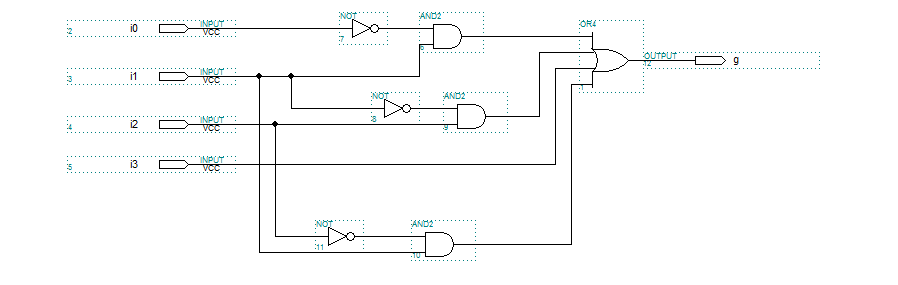
\includegraphics[scale=0.7]{dec_g.png}
  \caption{Decodificador 'g'}
\end{figure}

\FloatBarrier
\section{Simulação}

A simulação funcional foi organizada de modo a cobrir todas as combinações possiveis para ativar os dígitos de 0 a 9 (como pode ser conferido na tabela verdade da seção 2). O resultado é tal como segue na figura:

\begin{figure}[h!]
  \centering
  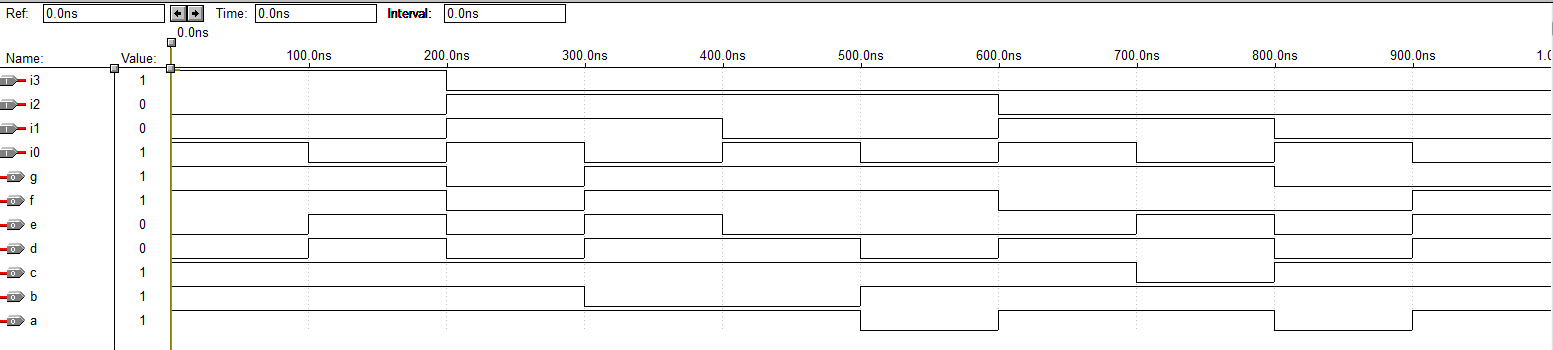
\includegraphics[scale=0.4]{simulacao.png}
  \caption{Simulação Funcional}
\end{figure}


\FloatBarrier

\section{Conclusão}
O experimento foi importante ao concretizar a noção  de otimização de circuitos através da minimização por mapas de Karnaugh. Entrentanto, nota-se que isto foi possível levando em conta que o projeto em questao é de um circuito relativamente simples e, para algo mais complexo, seria impraticável proceder desta maneira.

\end{document}
